\section{Dataset Processing}
\label{datasetprocessing}
\subsection{CT Image Data and Multimodal Data Generation}
\label{ctimagedata}
Because of the shortage of public CT dataset for pneumonia, we use raw data from the Radiology Department of The First Affiliated Hospital of Army Medical University. We get 1036 cases of CT(842 cases with pneumonia, 464 healthy cases) from hospital PACS(Picture Archiving and Communication Systems). Raw data from hospital may have more than one series of images, each series may have different data type, different image windows, or series with different angles. 
Generally speaking, radiologists and doctors will use series under lung window with smallest `Slice Thickness', but for deep learning models, we need to pick up the most suitable series manually. This work is very heavy, so we design a protocol to pick up series for us.

First of all, we eliminate these cases which start scanning from the middle of the chest. Then we pick up the best series from the whole cases according to the following requirements:

1. We use the series with the specific `Convolution Kernel'. Different `Convolution Kernel' may have different data types or differnet image windows, as shown in Fig~\ref{Bs}. We need to notice that these names of `Convolution Kernel' vary between hospitals and CT equipments, so if you want to adopt this protocol, you need to observe `Convolution Kernel' in your environment. In our study, we choose `B31f', `I31f 3', `B70f', `B80f', `B70s'. Number of different `Convolution Kernel' is shown in Fig~\ref{NumberofDifferentConvolutionKernel}. 
However, different `Convolution Kernel' will not affect images we analyze in the end, because all slices will be calculated and transformed into HU value matrices, which will be discussed later in this section.

\begin{figure}[t]
    \centerline{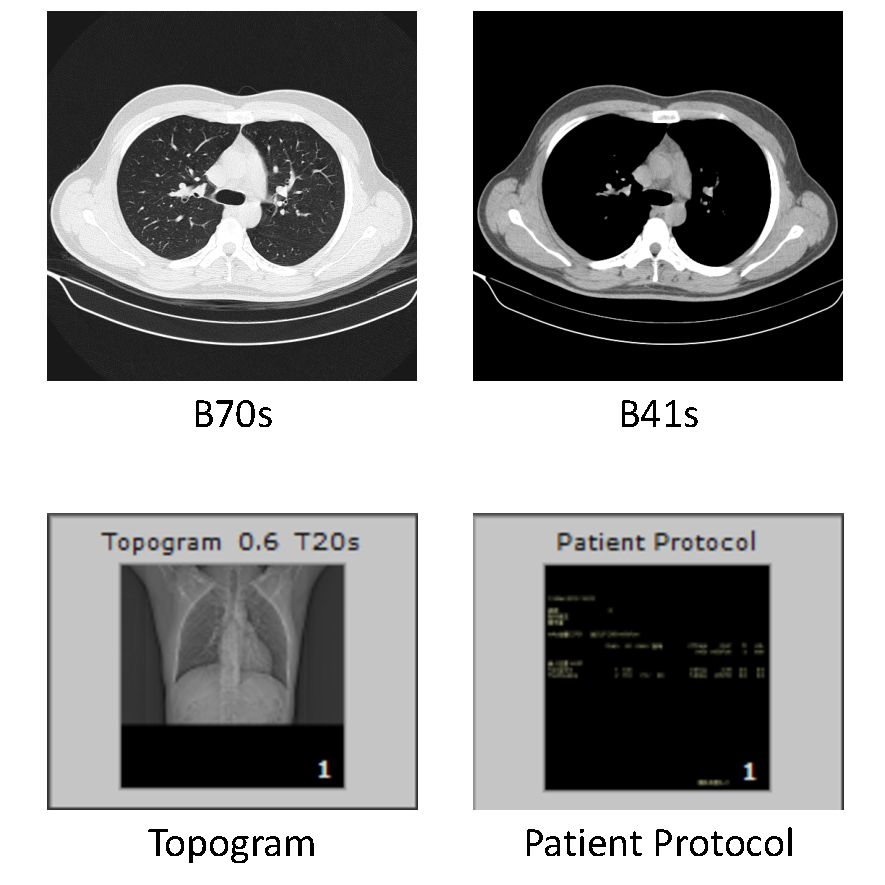
\includegraphics[width=90mm]{Bs.pdf}}
    \vspace{-0cm}
    \caption{Scans under Different `Convolutional Kernel'. Slice under `B70s' has clearer view of lungs, slice under `B41s' has clearer view of heart. `Patient Protocol' and `Topogram' contain some basic parameters of CT equipments or information about radiologists, which are not suitable for CNN.}
    \vspace{-0cm}
    \label{Bs}
    \end{figure}

2. We remove series which are not showing cross section of human body like `Patient Protocol', `Topogram'. `Patient Protocol' and `Topogram', as shown in Fig~\ref{Bs}, contain some basic parameters of CT equipments or information about radiologists, which should be eliminated.

3. We calculate `Slice Thickness' of each series, and keep series with the smallest `Slice Thickness', since small thickness may keep more detailed information of body structure. 

4. If there were more than one series meet the last two requirements, we will keep the series with the largest number of slices, which can have a larger span of view.

As a result, we keep 552 pneumonic cases and 450 cases of healthy people (1002 cases total).
We split dataset in training/validation/testing as 60\% / 20\% / 20\% and make them identically distributed in three parts of datasets, so we have 602 cases in training set, 200 cases in validation set, 200 cases in test set.
Number of healthy and pneumonic cases in different slice-thickness is shown in Table~\ref{distributionofhealthyandpneumonic}.

Each CT scan has a case file. In case files, we can get patient basic information: patient ID, gender, age and complaint. 

\begin{figure}[t]
\centerline{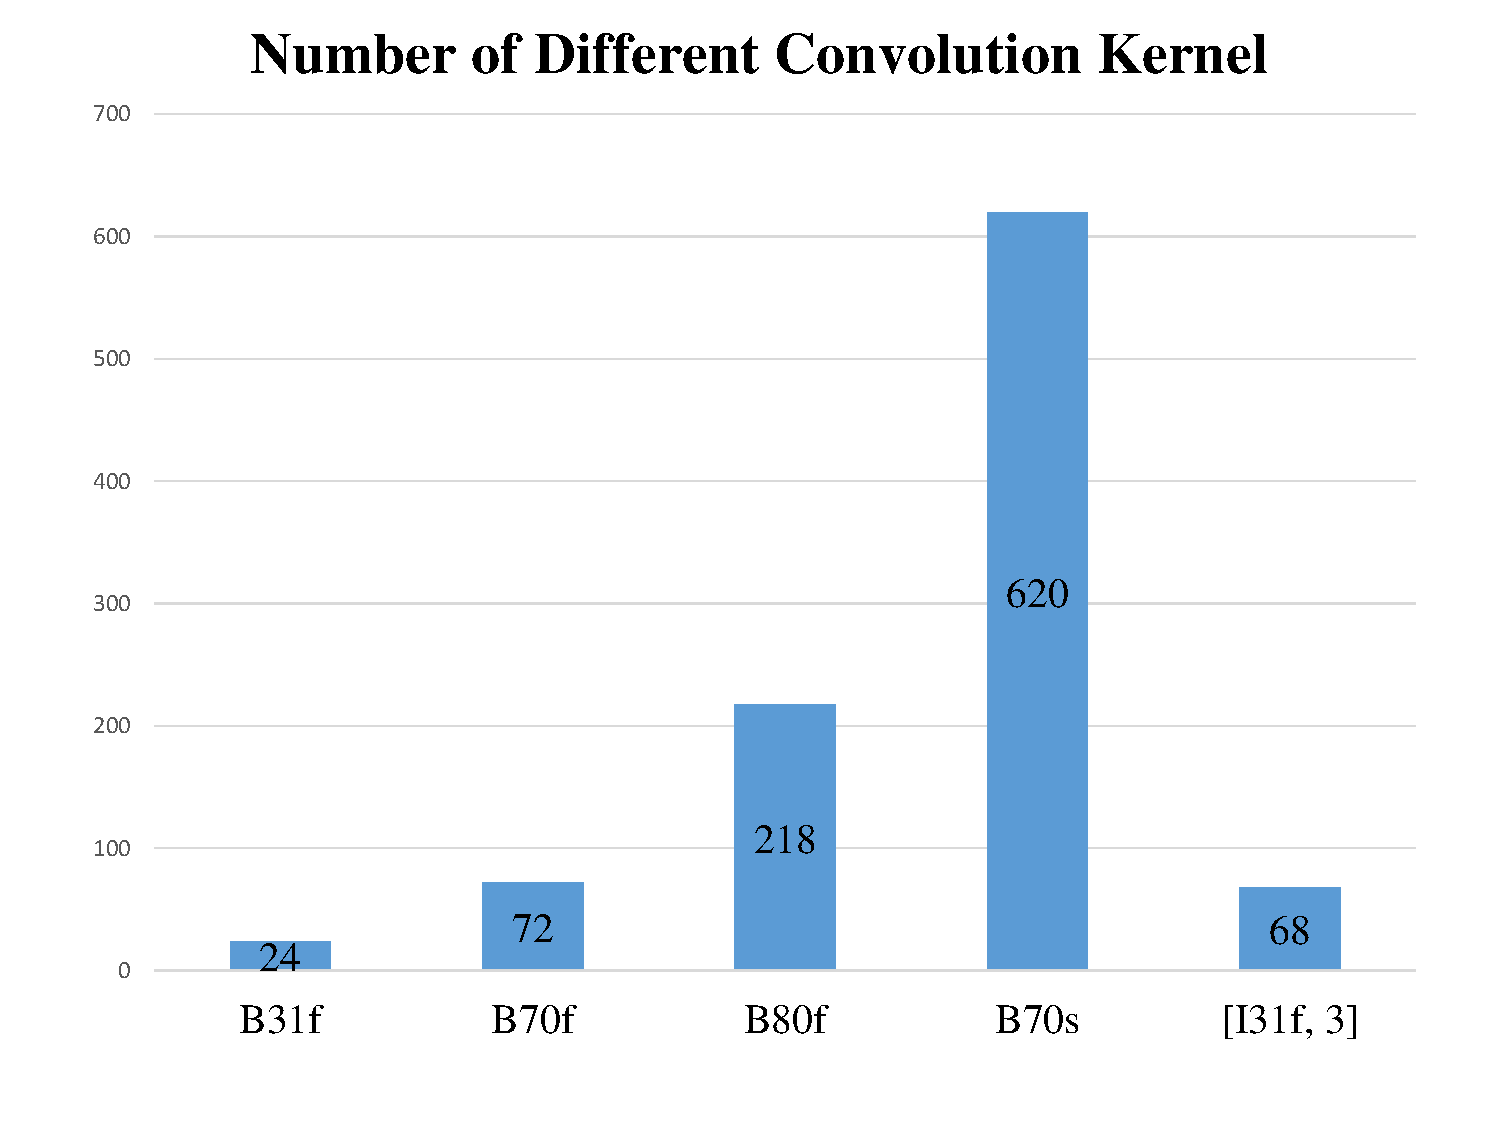
\includegraphics[width=100mm]{NumberofDifferentConvolutionKernel.pdf}}
\vspace{-0cm}
\caption{Number of Different `Convolution Kernel'. We notice that in the Radiology Department of The First Affiliated Hospital of Army Medical University, `B70s' is the most common parameter used in clinical. However, this parameter varys between hospitals and clinics.}
\vspace{-0cm}
\label{NumberofDifferentConvolutionKernel}
\end{figure}


\begin{table}[htb]
\vspace{-0cm}
\caption{Number of Healthy and Pneumonic Cases in Different Slice-Thickness}
\vspace{-0cm}
\begin{center}
\begin{tabular}{|c|c|c|}
\hline
\textbf{\textit{Slice-Thickness}}& \textbf{\textit{Healthy}}& \textbf{\textit{Pneumonic}}  \\
\hline
1 mm & 0 & 24 \\
1.5 mm  & 1 & 7\\
2 mm & 444 & 386  \\
3 mm & 0 & 127  \\
5 mm & 5 & 8  \\
\hline
Total & 450 & 552 \\
\hline
\end{tabular}
\vspace{-0cm}
\label{distributionofhealthyandpneumonic}
\end{center}
\vspace{-0cm}
\end{table}

\subsubsection{Pre-processing of CT Image Data}
\label{ctimagedata}
There are kinds of image windows for CT reader, such as windows for bone, brain, chest, lungs. Images under different image windows will highlight different tissues of bodies.
As mentioned in section\ref{ctimagedata}, we can see that each series of CT actually has one specific `Convolution Kernel' and show specific window for CT images directly from raw data. But it may make data inconsistent between different cases. So we transform raw data into HU(Hounsfield Unit) values. The Hounsfield Unit named after Sir Godfrey Hounsfield, is a quantitative scale for describing radio-density, its value is also termed CT number. After transformed into HU value matrices, all slices form CT scans will have the same unit of measure, then we will transform scans according to specific rules.

Following the study in \cite{Shin2017Three} \cite{gao2018holistic}, slices will be transformed into images using three HU range: Lung Window(LW) [-1000, 400HU], High Attenuation(HA) [-160, 240HU], Low Attenuation(LA) [-1400, -950HU]. 
For each slice, it will generate three one-channel grey level images(LW, HA, LA). Then we compress three one-channel grey level images into one three-channel false color RGB image. The `Slice Thickness' between each slice is adjusted into 10mm, and each case will keep 32 slices.

As shown in Fig~\ref{3channel}, we can clearly see that three-channel images can show more density information about lung tissues. Original CT images are actually grey level images, which can only show lungs with white, black or grey. In original CT images, high dense tissues are white, normal lung tissues and low dense tissues are tend to be black. If you want to see details of low dense tissues, you have to adjust the image window to low attenuation range, but meanwhile you will lost the details of high dense tissues. 
In three-channel images, details of high dense and low dense tissues will both be kept. Three-channel fake color images have a larger scale of colors. First of all, high dense tissues will still tend to be white, like bones, high dense tissues in lungs. Second, normal lung tissues will tend to be red, low dense tissues tend to be black, which is very useful when patients have severe lung diseases.
The influence of different HU value ranges will be discussed in section~\ref{effectiveness}.

\begin{figure*}[!t]
    \centerline{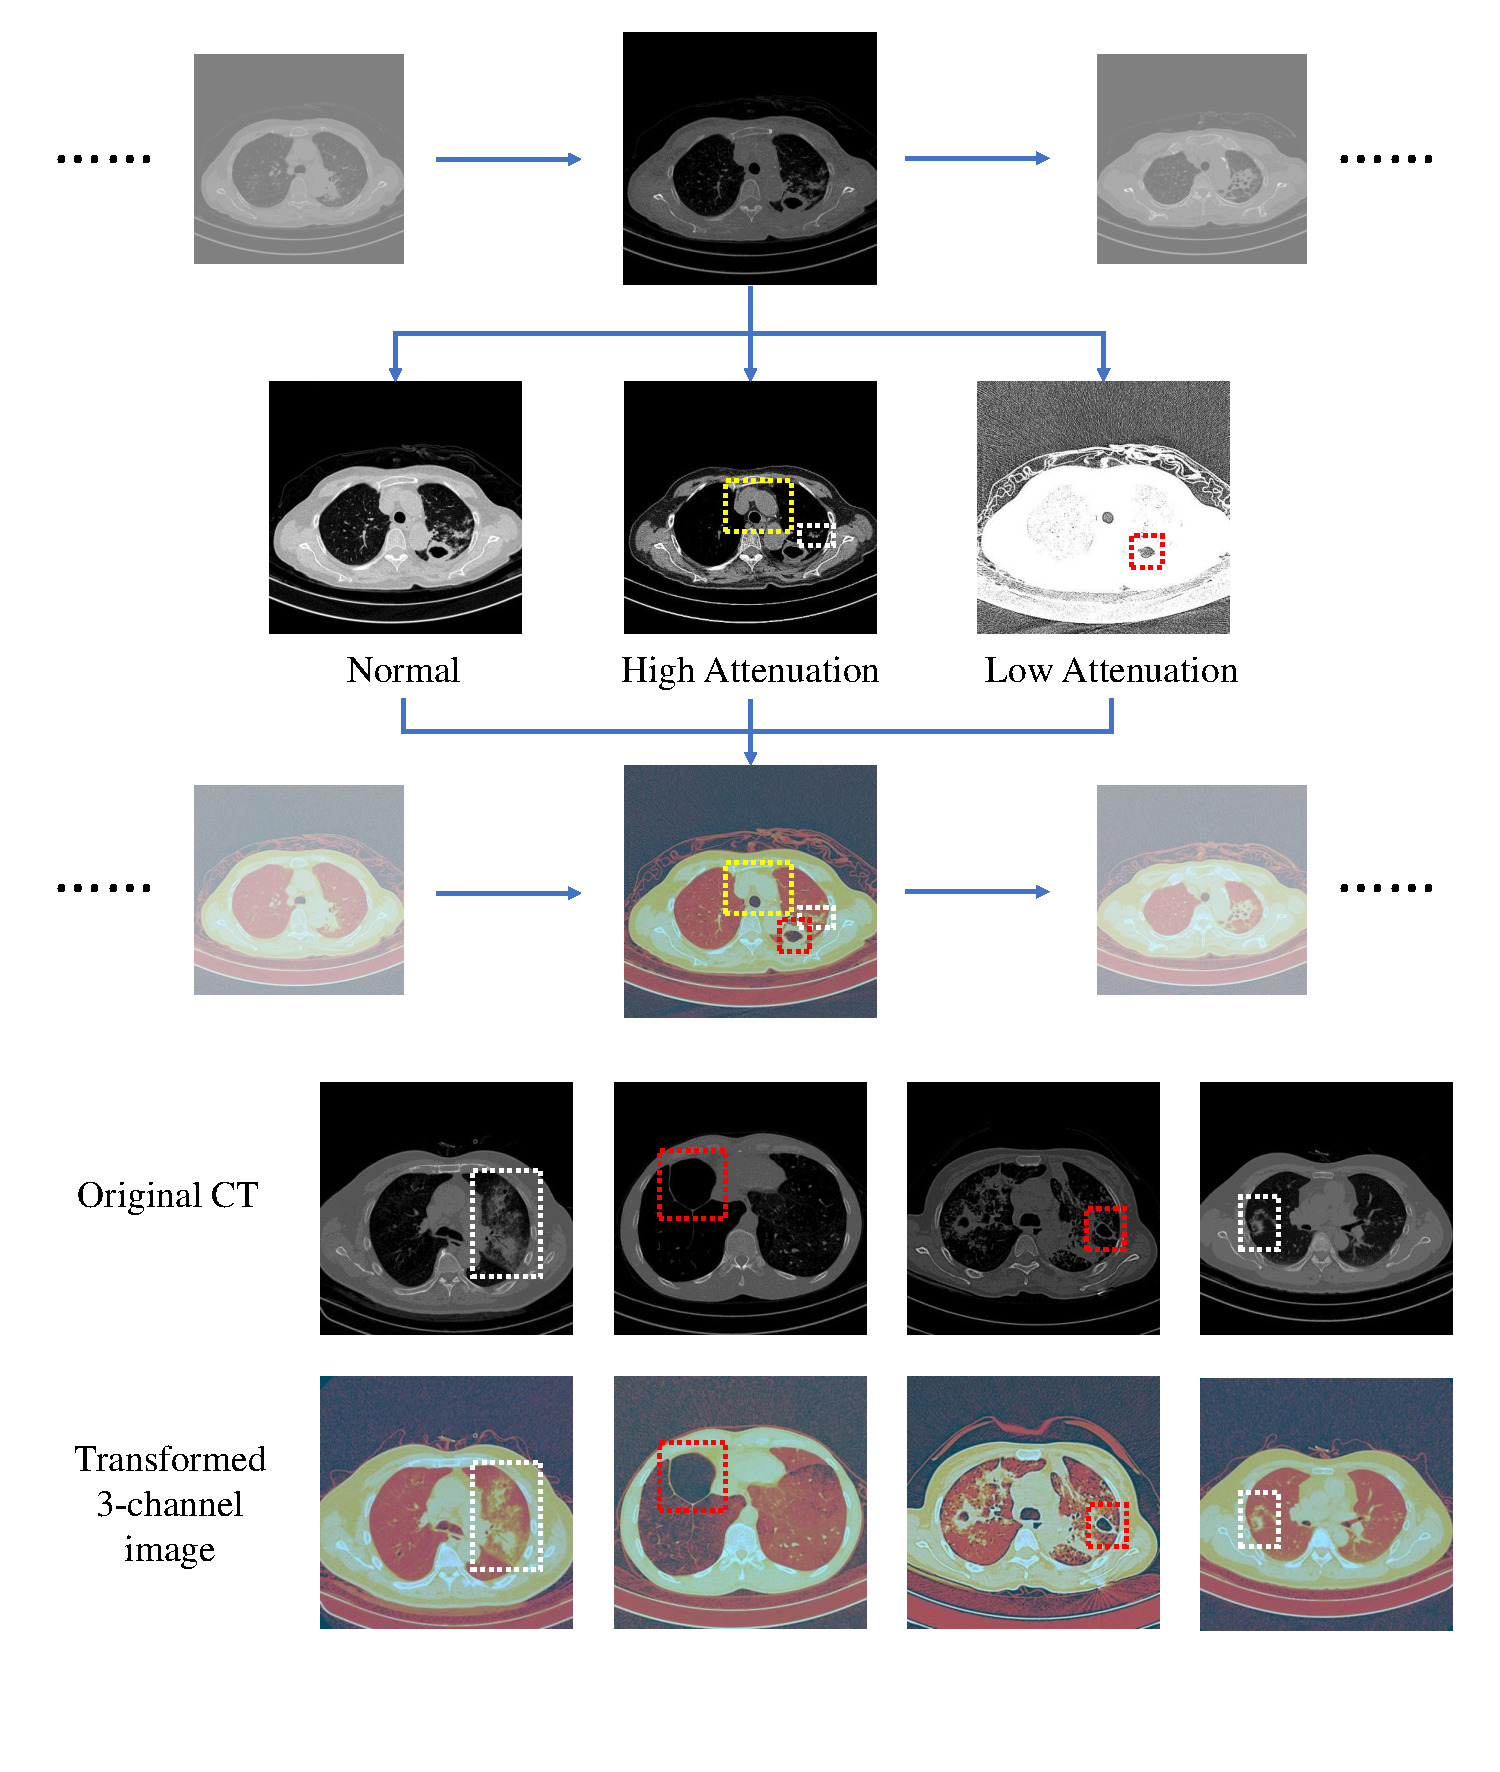
\includegraphics[width=150mm]{3channel.pdf}}
    \vspace{-1cm}
    \caption{Data Pre-precess for CT Scans. Void space(in red rectangle) in original CT images is not very obvious since other normal tissues is in black color too. But in three-channel image, we can clearly notice the difference between normal tissues and low dense tissues. Moreover, the details of high dense tissues(in white rectangle) are still kept. }
    \vspace{-0cm}
    \label{3channel}
    \end{figure*}

\subsubsection{Pre-processing of Patient Age, Gender and Complaints}
\label{textdata}
The pre-process steps of age, gender and complaints is shown in Fig~\ref{textinfo}. 
For patient age and gender, we transform them into a two-dimensional array. For example, patient in \ref{textinfo} is an adult male, who was born in 1999-10-29. His gender and age will be transformed to $[1, 20]$. A female patient born in 1993 will have $[0, 26]$ to represent her information. $1$ represents male patient, $0$ represents female patient.

For patients' complaints, since we only have Chinese complaints, we have to do Chinese word segmentation. Chinese word segmentation is a very difficult problem so we will take a short cut and use a mature tools: Jieba text segmentation to segment Chinese sentences into Chinese word sequences. An example of Chinese word segmentation is shown in green rectangle in Fig~\ref{textinfo}.
After word segmentation, we use word2vec \cite{mikolov2013efficient} \cite{mikolov2013distributed} to embed word sequences into vectors and use CBOW(Continuous Bag-of-Words) to keep relationship between words. Since our corpus is very small, we set embedding size as 50, and window size for CBOW as 3. In order to simplify model, we set length of Chinese word sequence to 16 since 16 is the maximum length among all complaint sequences. For those sequences whose length is less than 16, we add `None' to fill up the voids and increas length to 16. The details of word2vec will not be discussed here. After embedding, each word will be embedded into a vector of 50 dimensions.
\begin{figure}[!t]
    \centerline{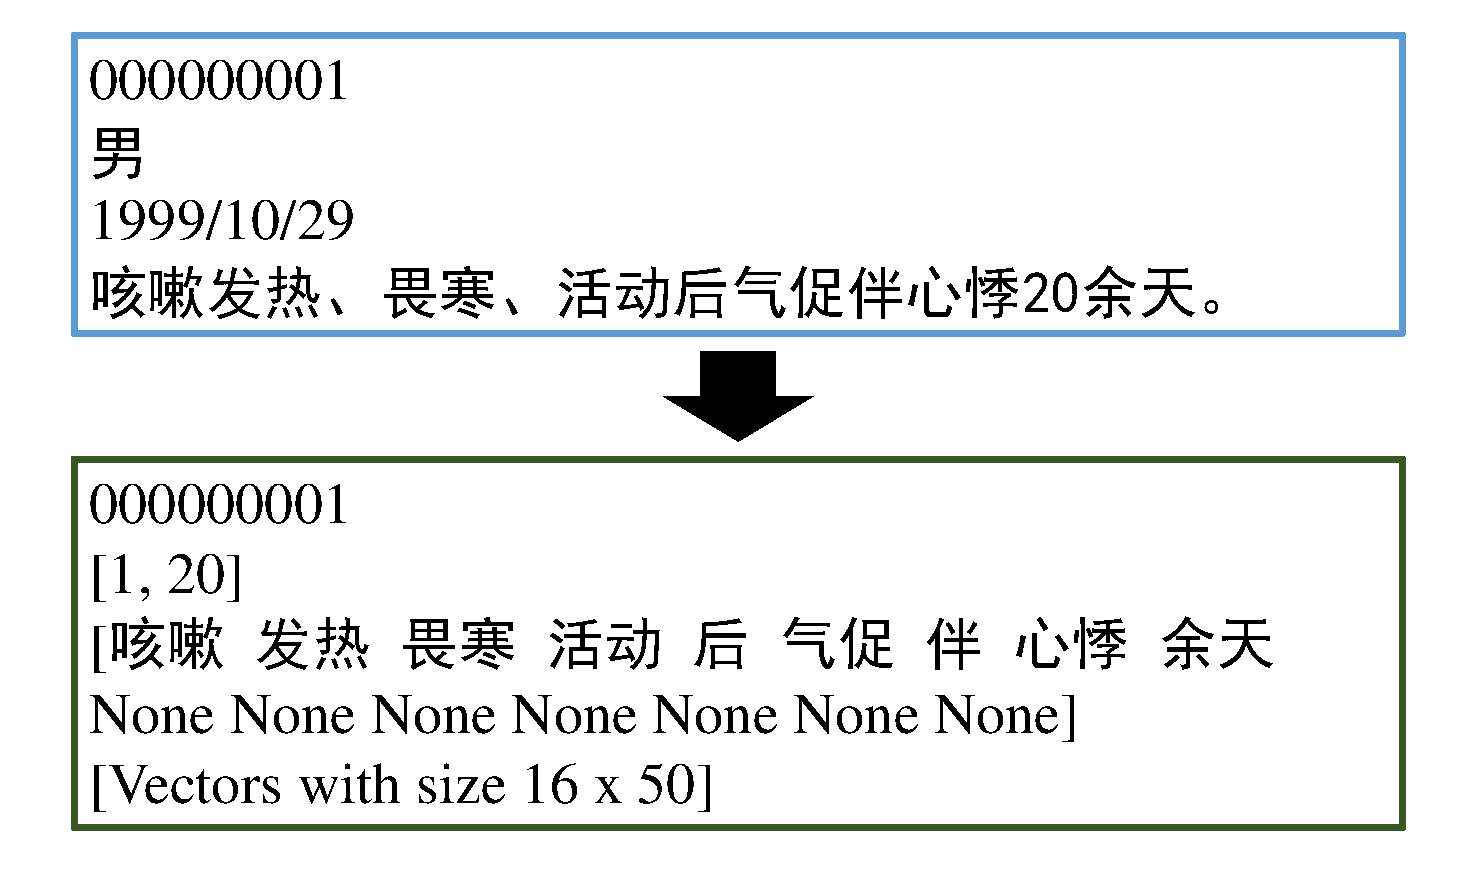
\includegraphics[width=90mm]{textinfo.pdf}}
    \vspace{-0cm}
    \caption{Data Pre-precess for Age, Gender and Complaints}
    \vspace{-0cm}
    \label{textinfo}
    \end{figure}